\chapter{Problemdomäne Pressenplanung}
\label{chapter:problem}
In diesem Kapitel wird das Problem der Pressenplanung zunächst erläutert,
bevor die prädikatenlogische Modellierung des Problems in einem Modell erfolgt.
Abschließend wird das Modell um Optimierungsziele erweitert.

\section{Anforderungen}
\label{sec:anforderungen}
Im Pressenplanungsproblem sind drei Entitäten und deren Eigenschaften von elementarer Bedeutung: Pressen, Balken und Bauteile.
Diese haben jeweils die Eigenschaften Höhe, Breite und Länge.
Zusätzlich gibt es Holzlamellen, welche durch Zersägen eines sogenannten \textit{Endlosbretts} entstehen.
Dieses kann von einer Maschine \textit{scheinbar} endlos ausgegeben werden.
Höhe und Breite der Lamelle sind fest.
Lamellen werden vertikal zu Bauteilen verleimt, sodass Bauteile immer die Form eines Quaders haben.
Diese Verleimung ist der eigentliche Grund für die Notwendigkeit des Pressens.
Folgend eine Abbildung verleimter Lamellen:

\begin{figure}[h]
    \centering
    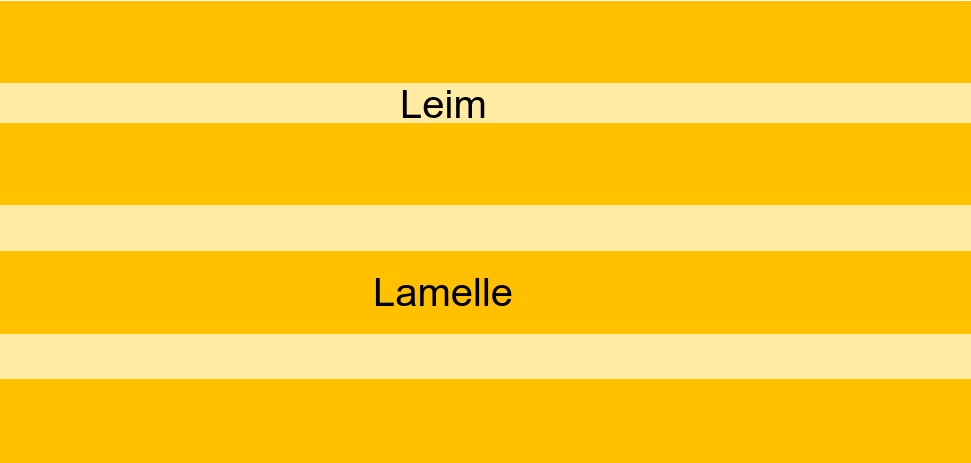
\includegraphics[width=0.70\textwidth, center]{Images/LammelleLeim}\\
    \caption{Vertikale Verleimung von Lamellen}
    \label{figure:lamelleleim}
\end{figure}

Bauteile wiederum formen Balken - ebenfalls Quader.
Bauteile erhält man durch vertikales Zersägen eines Balkens.
Folgend eine Abbildung eines Balkens aus drei Bauteilen mit Rest:

\begin{figure}[h]
    \centering
    
\includegraphics[width=1.00\textwidth, center]{Images/BalkenBauteileRest}\\
    \caption{Balken aus drei Bauteilen mit Rest, Sägelinien schwarz gepunktet}
    \label{figure:balkenbauteilerest}
\end{figure}

Balken werden vertikal in Pressen gestapelt und anschließend gepresst.
Eine mit Balken befüllte Presse, bei der festgelegt ist, wie die Balken zu Bauteilen nach der Pressung zersägt werden müssen, nennt man auch Pressenplan.
In einem Pressenplan ist jedem Bauteil höchstens eine Position in einer Schicht (von unten gezählter Balken) einer Presse zugeordnet.
Folgend die Visualisierung eines Pressenplans für eine Presse:

\begin{figure}[h]
    \centering
    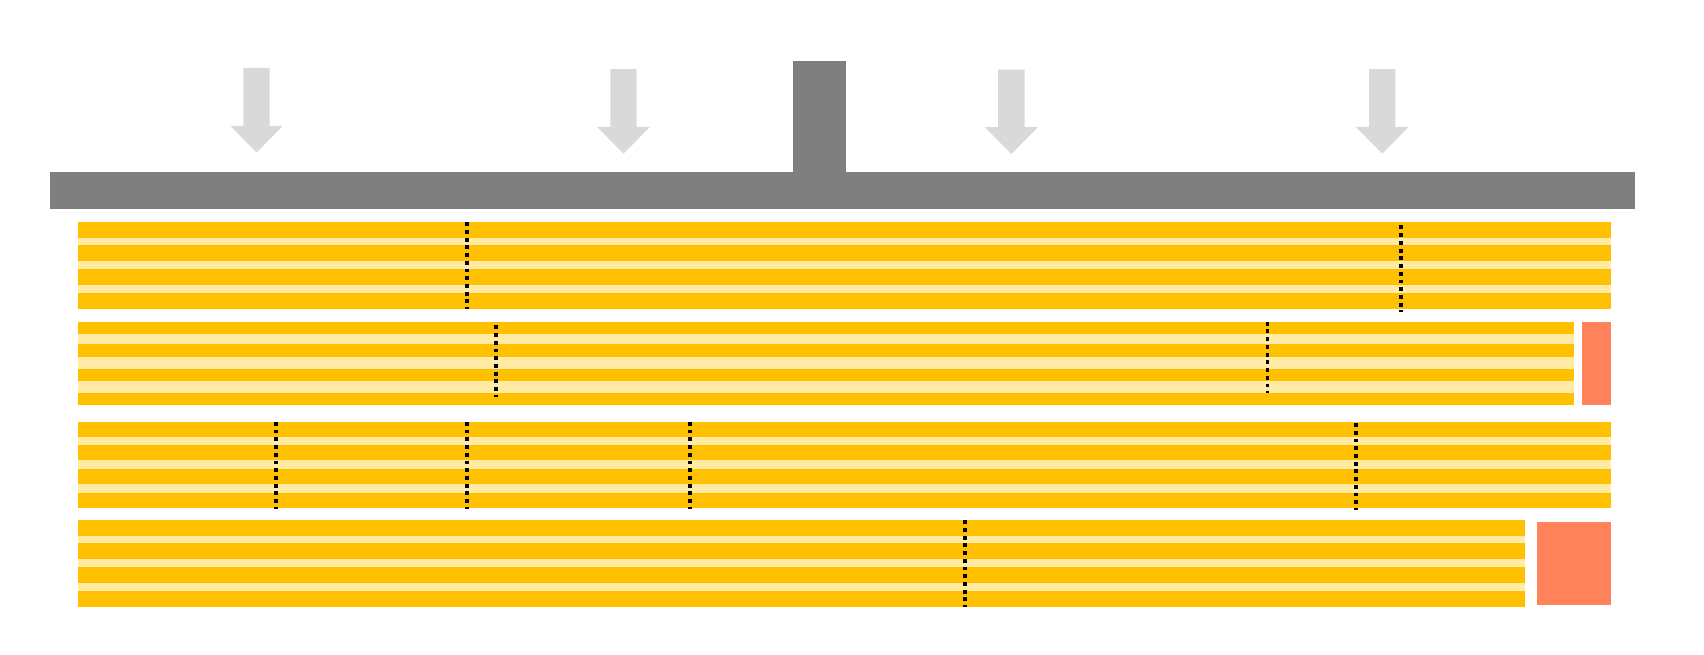
\includegraphics[width=1.00\textwidth, center]{Images/Pressenplan}\\
    \caption{Pressenplan für eine Presse mit vier Balken, 13 Bauteilen und zwei Reststücken}
    \label{figure:pressenplanproblem}
\end{figure}

Da Pressen im Allgemeinfall in einer Pressung nur Bauteile gleicher Breite pressen können, werden die Bauteile nach Breite vorsortiert.
Damit reduziert man die Dimension des Problems vom 3-Dimensionalen auf das 2-Dimensionale, da nur noch Länge und Höhe aller Entitäten berücksichtigt werden muss.

Die Eingabe für das Pressenplanungsproblem ist eine Liste von Bauteilen mit Länge und Höhe sowie deren Anzahl.
Diese Eingabe wird auch Auftrag genannt.
Folgend ein beispielhafter Auftrag:

\begin{table}[H]
    \centering
    \begin{tabular}{|c|c|c|}
        \hline
        \textbf{Länge in mm} & \textbf{Höhe in mm} & \textbf{Anzahl} \\
        \hline
        7000 & 400 & 1 \\
        13000 & 400 & 2 \\
        3000 & 400 & 3 \\
        6000 & 400 & 1 \\
        9000 & 400 & 1 \\
        7500 & 400 & 1 \\
        5000 & 400 & 1 \\
        5500 & 400 & 1 \\
        3500 & 400 & 1 \\
        \hline
    \end{tabular}
    \caption{Beispielauftrag, jede Zeile entpricht einer Bauteilspezifikation}
    \label{tab:auftrageingabe}
\end{table}

Die Lösung des Pressenplanungsproblems (Ausgabe) ist ein Pressenplan.
Für den Auftrag in Tabelle \ref{tab:auftrageingabe} könnte beispielsweise folgende Ausgabe den Pressenplan beschreiben:

\begin{table}[H]
    \centering
    \begin{tabular}{|c|c|c|c|c|}
        \hline
        \textbf{Presse} & \textbf{Schicht} & \textbf{Position} & \textbf{Länge in mm} & \textbf{Höhe in mm} \\
        \hline
        1 & 1 & 1 & 14000 & 400 \\
        1 & 1 & 2 & 7500 & 400 \\
        1 & 2 & 1 & 3000 & 400 \\
        1 & 2 & 2 & 6500 & 400 \\
        1 & 2 & 3 & 3000 & 400 \\
        \ldots & \ldots & \ldots & \ldots & \ldots \\
        \hline
    \end{tabular}
    \caption{Beispielausgabe des Pressenplans zu Auftrag in Tabelle \ref{tab:auftrageingabe}, Visualisierung in Abbildung \ref{figure:pressenplanproblem}}
    \label{tab:auftragausgabe}
\end{table}

An einen Pressenplan bestehen folgende Anforderungen:
\begin{enumerate}
    \item Pressen haben eine Minimal- und Maximalhöhe. Die Summe der Höhe aller Balken einer Presse muss in diesem Intervall liegen.
    \item Pressen haben eine Minimal- und Maximallänge. Die Länge aller Balken einer Presse muss in diesem Intervall liegen.
    \item Alle Balken einer Presse haben die gleiche Länge. Dazu kann der Balken so aus Bauteilen zusammengesetzt sein, dass ein Rest übrig bleibt.
    \item Alle Bauteile, die einen Balken formen, haben die gleiche Höhe.
    \item Jedes Bauteil eines Auftrages ist höchstens einem Balken zugeordnet.
    \item Jeder Balken ist genau einer Presse zugeordnet.
\end{enumerate}

\section{Modellierung}
\label{sec:modellierung}
In diesem Abschnitt wird das Modell zur Modellierung des Pressenplanungsproblems erläutert.
Alle Namen von Funktionen in jenem Modell werden englisch formuliert, um die Nähe zur später in Abschnitt \ref{sec:kodierungconstraints} gezeigten Implementierung zu wahren.
Pressen heißen also \textit{Press}, Balken (Schichten) werden \textit{Layer} genannt und Bauteile erhalten den Namen \textit{Component}.
Die Menge aller Pressen wird mit $P$, die Menge aller Schichten mit $L$ und die Menge aller Bauteile mit $C$ abgekürzt.

Betrachten wir für das Modell die Signatur $\Sigma = \left( \Sigma_F, \Sigma_R \right)$ und die Unbekannten $\mathbb{X} = (\mathbb{X}_{\mathbb{B}}, \mathbb{X}_{\mathbb{N}_0})$.
Jede Presse hat sowohl Minimal- und Maximallänge als auch Minimal- und Maximalhöhe.
Weiter wird jeder Presse eine Menge an Schichten zugeordnet.
Tatsächliche Länge und Höhe der Presse sind unbekannt:
\[
    \begin{array}{lll}
        \begin{aligned}
            \Sigma_{F}^{P} = \left\{
            \begin{aligned}
                & \text{minLength}: & P \rightarrow \mathbb{N}_0, \\
                & \text{maxLength}: & P \rightarrow \mathbb{N}_0, \\
                & \text{minHeight}: & P \rightarrow \mathbb{N}_0, \\
                & \text{maxHeight}: & P \rightarrow \mathbb{N}_0, \\
                & \text{layers}: & P \rightarrow 2^{L} \; \\
            \end{aligned} \right\} \\[5pt]
        \end{aligned}
        &
        \begin{aligned}
            \mathbb{X}_{\mathbb{N}_0}^{P} &= \left\{
                \begin{aligned}
                    & \text{length}: & P \rightarrow \mathbb{N}_0, \\
                    & \text{height}: & P \rightarrow \mathbb{N}_0 \; \\
                \end{aligned} \right\}
        \end{aligned}
        &
        \begin{aligned}
            \mathbb{X}_{\mathbb{B}}^{P} &= \emptyset
        \end{aligned}
    \end{array}
\]
Für die Zuordnung der Schichten zu den Pressen wird eine disjunkte Aufteilung aller Schichten gefordert:
\begin{align}
    L = \dot{\bigcup_{\substack{p \in P}}} \text{layers}(p) \label{constraint:disjointLayers}
\end{align}
Schichten haben unbekannte Länge, Höhe, einen unbekannten Rest und eine boolesche Unbekannte, welche kennzeichnet, ob eine Schicht leer ist:
\[
    \begin{array}{lll}
        \begin{aligned}
            \Sigma_{F}^{L} = \emptyset \\[5pt]
        \end{aligned}
        &
        \begin{aligned}
            \mathbb{X}_{\mathbb{N}_0}^{L} &= \left\{
            \begin{aligned}
                & \text{length}: & L \rightarrow \mathbb{N}_0, \\
                & \text{height}: & L \rightarrow \mathbb{N}_0, \\
                & \text{waste}: & L \rightarrow \mathbb{N}_0 \; \\
            \end{aligned} \right\}
        \end{aligned}
        &
        \begin{aligned}
            \mathbb{X}_{\mathbb{B}}^{L} &= \left\{ \text{isEmpty}: L \rightarrow \mathbb{B} \right\}
        \end{aligned}
    \end{array}
\]
Komponenten werden konkrete Längen und Höhen zugeordnet:
\[
    \begin{array}{lll}
        \begin{aligned}
            \Sigma_{F}^{C} = \left\{
            \begin{aligned}
                & \text{length}: & C \rightarrow \mathbb{N}_0, \\
                & \text{height}: & C \rightarrow \mathbb{N}_0 \; \\
            \end{aligned} \right\} \\[5pt]
        \end{aligned}
        &
        \begin{aligned}
            \mathbb{X}_{\mathbb{N}_0}^{C} &= \emptyset
        \end{aligned}
        &
        \begin{aligned}
            \mathbb{X}_{\mathbb{B}}^{C} &= \emptyset
        \end{aligned}
    \end{array}
\]
Zudem soll eine Relation die Zuordnung von Komponenten zu Schichten beschreiben:
\[
    \Sigma_{R} = \left\{ \text{InLayer} \subseteq C \times L \right\}
\]
Da diese allerdings unbekannt ist, wird die Relation durch eine unbekannte Funktion repräsentiert:
\[
    \mathbb{X}_{\mathbb{B}}^{\text{InLayer}} = \left\{ \text{InLayer}: C \times L \rightarrow \mathbb{B} \right\}
\]
Insgesamt ergibt das also folgende Signatur:
\begin{align*}
    &\hspace{0pt} \Sigma = \left( \Sigma_F, \Sigma_R \right) \text{ mit } \\
    &\hspace{20pt} \Sigma_F = \Sigma_{F}^{P} \cup \Sigma_{F}^{L} \cup \Sigma_{F}^{C} \\
    &\hspace{20pt} \Sigma_R = \emptyset \\
    &\hspace{0pt} \mathbb{X} = (\mathbb{X}_{\mathbb{B}}, \mathbb{X}_{\mathbb{N}_0}) \text{ mit} \\
    &\hspace{20pt} \mathbb{X}_{\mathbb{B}_{\phantom{0}}} = \mathbb{X}^{P}_{\mathbb{B}} \cup \mathbb{X}^{L}_{\mathbb{B}} \cup \mathbb{X}^{C}_{\mathbb{B}} \cup \mathbb{X}^{\text{InLayer}}_{\mathbb{B}} \\
    &\hspace{20pt} \mathbb{X}_{\mathbb{N}_0} = \mathbb{X}^{P}_{\mathbb{N}_0} \cup \mathbb{X}^{L}_{\mathbb{N}_0} \cup \mathbb{X}^{C}_{\mathbb{N}_0}
\end{align*}

Die Anforderungen an einen Presseplan werden damit folgend realisiert:
\begin{align}
    & \forall p \in P: \text{minHeight}(p) \leq \text{height}(p) \leq \text{maxHeight}(p) \label{constraint:pressHeight} \\[10pt]
    & \forall p \in P: \text{minLength}(p) \leq \text{length}(p) \leq \text{maxLength}(p) \label{constraint:pressLength} \\[10pt]
    & \forall p \in P,\; \forall l \in \text{layers}(P): \neg \text{isEmpty}(l) \rightarrow \text{length}(p) = \text{length}(l) \label{constraint:layerLength} \\[10pt]
    & \forall c \in C,\; \forall l \in L: \text{InLayer}(c,l) \rightarrow \text{height}(c) = \text{height}(l) \label{constraint:layerHeight} \\[10pt]
    & \forall c \in C,\; \exists! l \in L: \text{InLayer}(c,l) \label{constraint:eoLayer} \\[10pt]
    & \forall l \in L: \text{isEmpty}(l) \leftrightarrow \neg\bigvee_{c \in C} \text{InLayer}(c,l) \label{constraint:emptyLayer1} \\[10pt]
    & \forall l \in L: \text{isEmpty}(l) \leftrightarrow (\text{length}(l) = 0 \land \text{height}(l) = 0) \label{constraint:emptyLayer2} \\[10pt]
    & \forall p \in P: \text{height}(p) = \sum_{\substack{l \in \text{layers}(p)}} \text{height}(l) \label{constraint:computePressHeight} \\[10pt]
    & \forall l \in L: \text{length}(l) = \text{waste}(l) + \sum_{\substack{c \in C}}
    \begin{cases}
        \text{length}(c) & \text{, } \text{InLayer}(c,l) \\
        0 & \text{, sonst}
    \end{cases} \label{constraint:computeLayerLength}
\end{align}
Constraint \ref{constraint:pressHeight} erfüllt Anforderung 1 aus Abschnitt \ref{sec:anforderungen}, während Constraint \ref{constraint:pressLength} Anforderung 2 erfüllt.
Anforderung 3 wird durch Constraint \ref{constraint:layerLength} und Anforderung 4 durch Constraint \ref{constraint:layerHeight} abgedeckt.
Constraint \ref{constraint:eoLayer} verhärtet Anforderung 5 aus Optimierungszwecken, siehe Abschnitt \ref{sec:optimierung}.
Anforderung 6 ist in diesem Modell Konstruktionsvorschrift mit \ref{constraint:disjointLayers}.
Die Constraints \ref{constraint:emptyLayer1} und \ref{constraint:emptyLayer2} definieren, wann eine Presse leer ist.
Constraints \ref{constraint:computePressHeight} und \ref{constraint:computeLayerLength} liefern die Definition für Pressenhöhe und Schichtlänge.

Das Modell beschreibt unbekannte Funktionen und nutzt damit Prädikatenlogik höherer Ordnung.
Da die Mengen $P$, $L$ und $C$ endlich sind, ist auch der Definitionsbereich aller unbekannten Funktionen des Modells endlich.
Daher kann das Modell auf Prädikatenlogik erster Ordnung reduziert werden, indem die unbekannten Funktionen durch unbekannte Werte realisiert werden.
Folgend beispielhaft für Pressen:
\begin{align*}
    &\hspace{0pt} \mathbb{X}_{\mathbb{N}_0}^{P}\prime = \bigcup_{p \in P} \left\{\text{length}_p, \text{height}_p\right\} \\
    &\hspace{0pt} \text{length}(p) = \text{length}_p \\
    &\hspace{0pt} \text{height}(p) = \text{height}_p \\
    &\hspace{0pt} \Sigma_{F}^{P}\prime = \Sigma_{F}^{P} \cup \left\{ \text{length}, \text{height} \right\}
\end{align*}

Wird anstelle der Quantifizierung im Modell außerdem grundinstanziiert, dann beträgt die Anzahl numerischer Unbekannter
$\lvert \mathbb{X}_{\mathbb{N}_0} \rvert = 2 \lvert P \rvert + 3 \lvert L \rvert$ und die Anzahl boolescher Unbekannter
$\lvert \mathbb{X}_{\mathbb{B}} \rvert = \lvert L \rvert + \lvert C \rvert \cdot \lvert L \rvert$.
Die Anzahl Unbekannter steigt also linear in Abhängigkeit zur Eingabe.
Das gilt offensichtlich auch für Anzahl und Größe der Constraints.

Im Folgenden der Arbeit werden Aufträge als Constraint-Systeme betrachtet.
Dabei ist ein Auftrag $a \in A$ die Konjunktion aller Constraints für eine Eingabe:
$a = \ref{constraint:pressHeight} \land \ref{constraint:pressLength} \land \ldots \land \ref{constraint:computeLayerLength}$.
Die Menge aller Modelle (hier erfüllende Belegung) für ein solches $a$ wird dabei folgend notiert:
\[
    \text{Mod}(a) = \left\{
        (\mathcal{S}, (\beta_{\mathbb{N}_0}, \beta_{\mathbb{B}})) \middle|
            \begin{array}{l}
                \mathcal{S} = ((\mathbb{N}_0, \mathbb{B}), \llbracket \cdot \rrbracket_{(\mathbb{N}_0, \mathbb{B})}) \text{ ist } \Sigma\text{-Struktur}, \\
                \beta_{\mathbb{N}_0}: \mathbb{X}_{\mathbb{N}_0} \rightarrow \mathbb{N}_0, \\
                \beta_{\mathbb{B}_{\phantom{0}}}: \mathbb{X}_{\mathbb{B}_{\phantom{0}}} \rightarrow \mathbb{B}, \\
                \llbracket a \rrbracket_{(\mathcal{S}, (\beta_{\mathbb{N}_0}, \beta_{\mathbb{B}}))} = \text{True}
            \end{array}
    \right\}
\]
Zur Vereinfachung der Notation können die Interpretationsfunktionen $\beta_{\mathbb{N}_0}$ und $\beta_{\mathbb{B}}$ zusätzlich mit einem Modell indiziert werden.
\[
    \forall a \in A, \; \forall s \in \text{Mod}(a), s = (\mathcal{S}, (\beta_{\mathbb{N}_0}, \beta_{\mathbb{B}})): \beta_{\mathbb{N}_0}^s \equiv \beta_{\mathbb{N}_0} \land \beta_{\mathbb{B}}^s \equiv \beta_{\mathbb{B}}
\]
Weiter werden folgende Funktionen zu Aufträgen definiert:
\begin{align*}
    & \text{presses}: A \rightarrow 2^P, \text{ presses}(a) = P_a, \text{ wobei } P_a \text{ ist Menge aller Pressen in } a \\
    & \text{layers}: A \rightarrow 2^L, \text{ layers}(a) = L_a, \text{ wobei } L_a \text{ ist Menge aller Schichten in } a \\
    & \text{components}: A \rightarrow 2^C, \text{ components}(a) = C_a, \text{ wobei } C_a \text{ ist Menge aller Komponenten in } a \\
\end{align*}

\section{Optimierung}
\label{sec:optimierung}
Das obige Modell beschreibt beliebige Lösungen für das Problem der Pressenplanung.
Um den Kostenaufwand beim Pressen zu reduzieren, sind Pressenpläne zusätzlich nach folgenden Kriterien lexikografisch zu optimieren (Vorgabe Germanedge):
\begin{enumerate}
    \item $ \min \left( \left\lvert \left\{ c \in C \middle| \neg\bigvee\limits_{\substack{l \in L}} \text{InLayer}(c,l) \right\} \right\rvert \right) $
    \item $ \min (\lvert P \rvert) $
    \item $ \min \left(\sum\limits_{\substack{l \in L}} \text{waste}(l) \right) $
\end{enumerate}
Ziel 1 ist die Minimierung der Anzahl unverplanter Komponenten.
Dort ist das Optimum bestenfalls null, sodass alle Komponenten verplant sind.
Existiert eine solche Lösung immer?
Also:
\[
    \forall a \in A, \; \exists s \in \text{Mod}(a): 0 = \left\lvert \left\{ c \in \text{components}(a) \middle| \neg\bigvee\limits_{\substack{l \in \text{layers}(a)}} \beta_{\mathbb{B}}^{s}(\text{InLayer}(c,l)) \right\} \right\rvert
\]
Nein, denn es lässt sich ein einfaches Gegenbeispiel konstruieren:
\begin{align*}
    &\hspace{0pt} \text{Seien } P = \left\{ p_1, p_2 \right\} \text{ und } C = \left\{ c_1,c_2 \right\} \text{ mit } \\
    &\hspace{0pt} \text{height}(c_2) < \text{minHeight}(p_1) \leq \text{minHeight}(p_2) < \text{maxHeight}(p_2) < \text{height}(c_1) = \text{maxHeight}(p_1) \\
    &\hspace{0pt} \text{Dann muss } c_1 \text{ in } p_1 \text{ und damit } c_2 \text{ in } p_2 \text{ verplant werden.} \\
    &\hspace{0pt} \text{Das geht aber nicht, weil: } \text{height}(c_2) < \text{minHeight}(p_2)
\end{align*}
Wie Erfahrungsberichte und alle Testfälle in Kapitel \ref{chapter:auswertung} zeigen, existiert mit hoher Wahrscheinlichkeit aber eine Lösung, in welcher alle Bauteile verplant sind.
Da die Verplanung aller Bauteile mit Constraint \ref{constraint:eoLayer} bereits im Modell festgehalten ist, sind alle erfüllenden Belegungen des Modells
bezüglich Optimierungsziel 1 optimal.
In den wenigen Fällen, in welchen die minimale Anzahl unverplanter Bauteile größer als null ist, existiert im Modell aus Abschnitt \ref{sec:modellierung} keine Lösung.
Die korrekte Modellierung wäre hier anstelle des Constraints \ref{constraint:eoLayer} folgende:
\[
    \forall c \in C: \text{atMost}\left(1, \bigcup_{l \in L} \left\{ \text{InLayer}(c,l) \right\}\right)
\]
Dafür müsste aber zusätzlich nach Optimierungsziel 1 optimiert werden.
Aufgrund des damit einhergehenden signifikanten Performance-Verlusts bei der Lösung durch den SMT-Solver sowie der Seltenheit solcher Fälle,
wird in diesem Modell das Nicht-Finden dieser Lösungen hingenommen.
